\documentclass[aps,prb,twocolumn,superscriptaddress,preprintnumbers,amsmath,amssymb,floatfix]{revtex4}
%\documentclass[aps,prb,preprint,superscriptaddress,amsmath,amssymb,floatfix]{revtex4}
%\documentclass[aps,prl,onecolumn,groupedaddress,amsmath,amssymb,12pt]{revtex4}
\usepackage{graphicx}
\usepackage{ifthen}
\usepackage{dcolumn}% Align table columns on decimal point
\usepackage{bm}% bold math
\usepackage{multirow}
\usepackage{booktabs}
\usepackage{bm}% bold math
\usepackage{amsbsy}
\usepackage{amsmath}
\usepackage{amssymb}
\usepackage{subfigure}


%Definition of new commands
\newcommand{\f}[2]{\ensuremath{\frac{\displaystyle{#1}}{\displaystyle{#2}}}}
\newcommand{\lr}[1]{\langle{#1}\rangle}
\newcommand{\colv}[2] {\left(\begin{array}{c} #1 \\ #2 \end{array}\right)}
\renewcommand{\thefootnote}{\fnsymbol{footnote}}
\newcommand{\be} {\begin{eqnarray}}
\newcommand{\ee} {\end{eqnarray}}
%--------------------------------------------------------------------------
%EQ COMMANDS
%--------------------------------------------------------------------------
\newcommand{\two}{\mspace{-2.0mu}}
\newcommand{\four}{\mspace{-4.0mu}}
\newcommand{\plus}{\mspace{-4.5mu}+\mspace{-3.5mu}}
\newcommand{\minus}{\mspace{-4.5mu}-\mspace{-3.5mu}}
\newcommand{\pp}{'\mspace{-2.0mu}'}
\newcommand{\xlb}[4]{#1\ifthenelse{\equal{#2}{0}}{}{_{\alpha #2}}
\mspace{-2.0mu}\genfrac{(}{)}{0pt}{1}{\ifthenelse{\equal{#3}{0}}{0}{l #3}} 
{\ifthenelse{\equal{#4}{0}}{0}{b #4}}}

\newcommand{\xkv}[4]{#1\mspace{-5.0mu}\left(\mspace{-8.0mu}
\begin{smallmatrix}#2\four{}\four{}\mspace{-8.0mu}&\pmb{\kappa}#3\\&\nu 
#4\end{smallmatrix}\mspace{-5.0mu}\right)}

\newcommand{\evect}[6]{#1\mspace{-4.0mu}\left(\mspace{-8.0mu}
\begin{smallmatrix}#2\mspace{-8.0mu}&\pmb{\kappa} #3 &b #5\\&\nu #4 &
\alpha #6\end{smallmatrix}\mspace{-5.0mu}\right)}

\newcommand{\varmat}[8]{\mspace{-5.0mu}\left(\mspace{-8.0mu}
\begin{smallmatrix}\ifthenelse{\equal{#3}{0}}{\mspace{-8.0mu}&b_{#1}&b_{#2}
\\&\alpha_{#1}&\alpha_{#2}} {\ifthenelse{\equal{#7}{0}}{#1\mspace{-8.0mu}&
\pmb{\kappa}#2#3\mspace{-8.0mu}&\pmb{\kappa}#4#5\mspace{-8.0mu}&\pmb{\kappa}
#6\\&\nu#2&\nu#4&\nu#6} {#1\mspace{-8.0mu}&\pmb{\kappa}#2#3\mspace{-8.0mu}&
\pmb{\kappa}#4#5\mspace{-8.0mu}&\pmb{\kappa}#6#7\mspace{-8.0mu}&\pmb{\kappa}
#8\\&\nu#2&\nu#4&\nu#6&\nu#8}}\end{smallmatrix}\mspace{-5.0mu}\right)}

\newcommand{\EXP}[1]{\exp\mspace{-5.0mu}\left[#1\right]\mspace{-3.0mu}}

\newcommand{\tpp}[2]{\left(\mspace{-2.0mu}\xkv{\omega}{}{}{}#1\xkv{\omega}
{}{'}{'}#2\xkv{\omega}{}{\pp}{\pp}\mspace{-2.0mu}\right)}



%--------------------------------------------------------------------------
\newcommand{\SUM}[2]{\ifthenelse{\equal{#1}{0}}{\sum_{
\alpha_{#2},b_{#2},l_{#2}}^{3,n,N}} {\ifthenelse{\equal{#1}{1}}{\sum_{
\alpha_{#2},b_{#2}}^{3,n}}{\sum_{\pmb{\kappa}#2,\nu#2}^{N,3n}}}}

\newcommand{\SUMprime}[2]{\ifthenelse{\equal{#1}{0}}
{\sum_{\alpha_{#2},b_{#2},l_{#2}}^{3,n,N}} 
{\ifthenelse{\equal{#1}{1}}{\sum_{\alpha_{#2},b_{#2}}^{3,n}}
{\sum_{\pmb{\kappa}^{'}#2,\nu#2}^{N,3n}}}}

\newcommand{\SUMalpha}[2]{\ifthenelse{\equal{#1}{0}}
{\sum_{\alpha_{#2}}^{3}} {\ifthenelse{\equal{#1}{1}}
{\sum_{\alpha_{#2},b_{#2}}^{3,n}}{\sum_{\pmb{\kappa}#2,\nu#2}^{N,3n}}}}
%--------------------------------------------------------------------------
\newcommand{\SUMalphap}[2]{\ifthenelse{\equal{#1}{0}}
{\sum_{\alpha'_{#2}}^{3}} {\ifthenelse{\equal{#1}{1}}
{\sum_{\alpha'_{#2},b'_{#2}}^{3,n}}{\sum_{\pmb{\kappa}#2,\nu#2}^{N,3n}}}}

\newcommand{\SUMb}[2]{\ifthenelse{\equal{#1}{0}}{\sum_{b_{#2}}^{n}}
 {\ifthenelse{\equal{#1}{1}}{\sum_{\alpha_{#2},b_{#2}}^{3,n}}
{\sum_{\pmb{\kappa}#2,\nu#2}^{N,3n}}}}

\newcommand{\SUMbp}[2]{\ifthenelse{\equal{#1}{0}}{\sum_{b'_{#2}}^{n}}
 {\ifthenelse{\equal{#1}{1}}{\sum_{\alpha'_{#2},b'_{#2}}^{3,n}}
{\sum_{\pmb{\kappa}#2,\nu#2}^{N,3n}}}}

\newcommand{\SUMl}[2]{\ifthenelse{\equal{#1}{0}}{\sum_{l_{#2}}^{N}}
 {\ifthenelse{\equal{#1}{1}}{\sum_{\alpha_{#2},b_{#2}}^{3,n}}
{\sum_{\pmb{\kappa}#2,\nu#2}^{N,3n}}}}

\newcommand{\SUMlp}[2]{\ifthenelse{\equal{#1}{0}}{\sum_{l'_{#2}}^{N}}
 {\ifthenelse{\equal{#1}{1}}{\sum_{\alpha'_{#2},b'_{#2}}^{3,n}}
{\sum_{\pmb{\kappa}#2,\nu#2}^{N,3n}}}}

\newcommand{\abcdt}[5]{\mspace{-4.0mu}\left(\mspace{-8.0mu}
\begin{smallmatrix}&\ifthenelse{\equal{#1}{}}{a}{#1}&\ifthenelse
{\equal{#3}{}}{c}{#3}\\&\ifthenelse{\equal{#2}{}}{b}{#2}&\ifthenelse
{\equal{#4}{}}{d}{#4}\end{smallmatrix}\mspace{-2.0mu};\ifthenelse
{\equal{#5}{}}{t}{#5}\right)}

\newcommand{\abcd}[4]{\mspace{-4.0mu}\left(\mspace{-8.0mu}
\begin{smallmatrix}&\ifthenelse{\equal{#1}{}}{a}{#1}&\ifthenelse
{\equal{#3}{}}{c}{#3}\\&\ifthenelse{\equal{#2}{}}{b}{#2}&\ifthenelse
{\equal{#4}{}}{d}{#4}\end{smallmatrix}\mspace{-3.0mu}\right)}

\newcommand{\abt}[3]{\mspace{-4.0mu}\left(\mspace{-8.0mu}\begin
{smallmatrix}&\ifthenelse{\equal{#1}{}}{a}{#1} \\&\ifthenelse{
\equal{#2}{}}{b}{#2}\end{smallmatrix}\mspace{-2.0mu};
\ifthenelse{\equal{#3}{}}{t}{#3}\right)}

\newcommand{\ab}[2]{\mspace{-4.0mu}\left(\mspace{-8.0mu}
\begin{smallmatrix}&\ifthenelse{\equal{#1}{}}{a}{#1} \\&\ifthenelse
{\equal{#2}{}}{b}{#2}\end{smallmatrix}\mspace{-3.0mu}\right)}

\newcommand{\kvbat}{\mspace{-4.0mu}\left(\mspace{-8.0mu}
\begin{smallmatrix} &\pmb{\kappa} &b \\ &\nu &\alpha\end{smallmatrix}
\mspace{-2.0mu};t\right)}
%--------------------------------------------------------------------------
\newcommand{\kvbatp}{\mspace{-4.0mu}\left(\mspace{-8.0mu}
\begin{smallmatrix} &\pmb{\kappa} &b' \\ &\nu &\alpha'\end{smallmatrix}
\mspace{-2.0mu};t\right)}

\newcommand{\kvbaw}{\mspace{-4.0mu}\left(\mspace{-8.0mu}
\begin{smallmatrix} &\pmb{\kappa} &b \\ &\nu &\alpha\end{smallmatrix}
\mspace{-2.0mu};\omega\right)}

\newcommand{\kvbawp}{\mspace{-4.0mu}\left(\mspace{-8.0mu}
\begin{smallmatrix} &\pmb{\kappa} &b' \\ &\nu &\alpha'\end{smallmatrix}
\mspace{-2.0mu};\omega\right)}

\newcommand{\kvba}{\mspace{-4.0mu}\left(\mspace{-8.0mu}
\begin{smallmatrix} &\pmb{\kappa} &b \\ &\nu &\alpha\end{smallmatrix}
\mspace{-3.0mu}\right)}

\newcommand{\kvbap}{\mspace{-4.0mu}\left(\mspace{-8.0mu}
\begin{smallmatrix} &\pmb{\kappa}' &b \\ &\nu' &\alpha\end{smallmatrix}
\mspace{-3.0mu}\right)}
%--------------------------------------------------------------------------
\newcommand{\kpvba}{\mspace{-4.0mu}\left(\mspace{-8.0mu}
\begin{smallmatrix} &\pmb{\kappa}^{'} &b \\ &\nu &\alpha\end{smallmatrix}
\mspace{-3.0mu}\right)}

\newcommand{\kva}{\mspace{-4.0mu}\left(\mspace{-8.0mu}
\begin{smallmatrix} &\pmb{\kappa} \\ &\nu &\alpha\end{smallmatrix}
\mspace{-3.0mu}\right)}

\newcommand{\kvap}{\mspace{-4.0mu}\left(\mspace{-8.0mu}
\begin{smallmatrix} &\pmb{\kappa} \\ &\nu &\alpha'\end{smallmatrix}
\mspace{-3.0mu}\right)}

\newcommand{\kvb}{\mspace{-4.0mu}\left(\mspace{-8.0mu}
\begin{smallmatrix} &\pmb{\kappa} &b \\ &\nu \end{smallmatrix}
\mspace{-3.0mu}\right)}

\newcommand{\kvbp}{\mspace{-4.0mu}\left(\mspace{-8.0mu}
\begin{smallmatrix} &\pmb{\kappa} &b' \\ &\nu \end{smallmatrix}
\mspace{-3.0mu}\right)}

\newcommand{\kvt}{\mspace{-4.0mu}\left(\mspace{-8.0mu}
\begin{smallmatrix}&\pmb{\kappa} \\&\nu\end{smallmatrix}
\mspace{-2.0mu};t\right)}

\newcommand{\kvzero}{\mspace{-4.0mu}\left(\mspace{-8.0mu}
\begin{smallmatrix}&\pmb{\kappa} \\&\nu\end{smallmatrix}
\mspace{-2.0mu};0\right)}

\newcommand{\kpvt}{\mspace{-4.0mu}\left(\mspace{-8.0mu}
\begin{smallmatrix}&\pmb{\kappa}^{'} \\&\nu\end{smallmatrix}
\mspace{-2.0mu};t\right)}

\newcommand{\kvw}{\mspace{-4.0mu}\left(\mspace{-8.0mu}
\begin{smallmatrix}&\pmb{\kappa} \\&\nu\end{smallmatrix}
\mspace{-2.0mu};\omega\right)}

\newcommand{\kv}{\mspace{-4.0mu}\left(\mspace{-8.0mu}
\begin{smallmatrix}&\pmb{\kappa} \\&\nu\end{smallmatrix}
\mspace{-3.0mu}\right)}

\newcommand{\kvp}{\mspace{-4.0mu}\left(\mspace{-8.0mu}
\begin{smallmatrix}&\pmb{\kappa'} \\&\nu'\end{smallmatrix}
\mspace{-3.0mu}\right)}

\newcommand{\kw}{\mspace{-4.0mu}\left(\mspace{-8.0mu}
\begin{smallmatrix}&\pmb{\kappa} \\&\omega\end{smallmatrix}
\mspace{-3.0mu}\right)}

\newcommand{\kpvp}{\mspace{-4.0mu}\left(\mspace{-8.0mu}
\begin{smallmatrix}&\pmb{\kappa'} \\&\nu'\end{smallmatrix}
\mspace{-3.0mu}\right)}
%--------------------------------------------------------------------------
\newcommand{\lbt}{\mspace{-4.0mu}\left(\mspace{-8.0mu}
\begin{smallmatrix}&l \\&b\end{smallmatrix}\mspace{-2.0mu};t\right)}

\newcommand{\lbtp}{\mspace{-4.0mu}\left(\mspace{-8.0mu}
\begin{smallmatrix}&l' \\&b'\end{smallmatrix}\mspace{-2.0mu};t\right)}

\newcommand{\lt}{\mspace{-4.0mu}\left(\mspace{-8.0mu}
\begin{smallmatrix}&l\end{smallmatrix}\mspace{-2.0mu};t\right)}

\newcommand{\ltp}{\mspace{-4.0mu}\left(\mspace{-8.0mu}
\begin{smallmatrix}&l'\end{smallmatrix}\mspace{-2.0mu};t\right)}

\newcommand{\lb}{\mspace{-4.0mu}\left(\mspace{-8.0mu}
\begin{smallmatrix}&l \\&b\end{smallmatrix}\mspace{-3.0mu}\right)}

\newcommand{\lbp}{\mspace{-4.0mu}\left(\mspace{-8.0mu}
\begin{smallmatrix}&l' \\&b'\end{smallmatrix}\mspace{-3.0mu}\right)}
%--------------------------------------------------------------------------
%COMMANDS
%--------------------------------------------------------------------------

%--------------------------------------------------------------------------
\begin{document}
%--------------------------------------------------------------------------

%--------------------------------------------------------------------------
\title{Evaluation of the Virtual Crystal Approximation for Predicting 
Thermal Conductivity}
%--------------------------------------------------------------------------
\author{Jason M. Larkin}
\affiliation{Department of Mechanical Engineering\\Carnegie Mellon 
University\\Pittsburgh, PA 15213}
\author{A. J. H. McGaughey}
\email{mcgaughey@cmu.edu}
\affiliation{Department of Mechanical Engineering\\
Carnegie Mellon University\\Pittsburgh, PA 15213}
%--------------------------------------------------------------------------

%--------------------------------------------------------------------------
\date{\today}
%--------------------------------------------------------------------------


%--------------------------------------------------------------------------
\begin{abstract}
%--------------------------------------------------------------------------
Accurately predicting the thermal conductivity of a dielectric or 
semiconducting material requires the properties of phonons from the entire 
Brillouin zone. Accurate predictions of phonon properties for bulk systems 
can be made with anharmonic lattice dynamics theory using ab initio 
calculations. However, computational costs limit the size of unit cells 
in ab initio calculations to be less than 100 atoms, making it difficult 
to directly incorporate the effects of disorder. Alternatively, theory 
that treats disorder as a harmonic perturbation can be used to estimate 
the reduction in phonon lifetimes due to disorder scattering without 
the use of a large unit cell. Under this approximation, the disordered
 crystal is replaced with a perfect “virtual crystal” with properties 
equivalent to an averaging over the disorder (e.g.  mass or bond 
strength). 
In this work, the virtual crystal approximation for mass disorder is 
evaluated by examining two model alloy systems: Lennard-Jones argon 
and Stillinger-Weber silicon. In both cases the perfect crystal is 
alloyed with a heavier mass species up to equal concentration . These 
two alloyed systems have different ranges of phonon frequencies, 
lifetimes, and mean free paths. For Stillinger-Weber silicon, the 
virtual crystal approximation predicts phonon properties and thermal 
conductivity in good agreement with molecular dynamics-based methods. 
For Lennard-Jones argon, the virtual crystal approximation underpredicts 
the high frequency phonon lifetimes, leading to an underpredicting of 
its thermal conductivity.
%--------------------------------------------------------------------------
\end{abstract}
%--------------------------------------------------------------------------


%--------------------------------------------------------------------------
\maketitle
%--------------------------------------------------------------------------
\clearpage
%--------------------------------------------------------------------------
\section{\label{S:Intro}Introduction}
%--------------------------------------------------------------------------

For thermolectric device applications, minimizing a thermoelectric 
material's thermal 
conductivity has become a promising technique for increasing $ZT>3$.
\cite{chen_recent_2003,dresselhaus_new_2007} In semiconductor alloys, 
understanding the effect of disorder is necessary for optimizing 
ZT by further lowering thermal conductivity.
\cite{he_thermoelectric_2006,huang_filler-reduced_2010,
toberer_phonon_2011,tian_phonon_2012}

Abeles first introduced the idea of using a virtual crystal (VC) to 
replace a disordered one by treating both
disorder and anharmonicity as perturbations.
\cite{abeles_lattice_1963} 
Recently, work using ab-initio calculations and the virtual crystal 
approximation \cite{garg_role_2011,tian_phonon_2012}.

The goal of this work is to verify the use of the virtual crystal 
approximation for predicting thermal conductivity by a detailed comparison 
of 3 methods for predicting thermal conductivity: MD-based normal mode 
decomposition (NMD) and green-kubo (GK), 
and anharmonic lattice dynamics (ALD) which treats the harmonic and 
anharmonic phonon scattering as perturbations. Two model alloy systems 
with mass defects are considered: 
Lennard-Jones argon and Stillinger-Weber silicon. 
In both cases the perfect crystal is 
alloyed with a heavier mass species up to equal concentration . These 
two alloyed systems have different ranges of phonon frequencies, 
lifetimes, and mean free paths. For Stillinger-Weber silicon, 
ALD predicts phonon properties and thermal 
conductivity in good agreement with MD-based methods NMD and GK. 
For Lennard-Jones argon, the VC approximation underpredicts 
the high frequency phonon lifetimes, leading to an underpredicting of 
its thermal conductivity. 

%--------------------------------------------------------------------------
\section{\label{S:}Virtual Crystal (VC) Approximation}
%--------------------------------------------------------------------------
Abeles introduced the idea of using a virtual (perfect) crystal 
to replace a disordered one, computing the
thermal conductivity of Si/Ge alloys by treating both
disorder and anharmonicity as perturbations.
\cite{abeles_lattice_1963} 
We calculate at all compositions
the phonon modes of the virtual crystal (which has
a lattice parameter, mass, and
force constants of that particular composition)
and derive from those the frequencies, group velocities,
and lifetimes to calculate thermal
conductivity.

Cahill shows that conductivty of dilute Ge-doped Si epitaxial layers
 agrees with 
a virtual crystal approximation with a phonon lifetime term that 
treats the defects as a peturbation (see section).
\cite{cahill_thermal_2004} 
Garg used ab initio calculations with anharmonic lattice dynamics (ALD) 
and the virtual crystal 
approximation (referred to as VC-ALD) 
to predict the thermal conductivity of Si-Ge alloys 
for all concentrations, obtaining good agreement with experiment.
\cite{garg_role_2011}  
A detailed study of PbTe/PbSe systems demonstrate the importance 
of bond environment for alloys.\cite{tian_phonon_2012} 

The computaitonal studies discussed above were limited to the use 
of VC-ALD because of the computational cost of ab initio calcualtions. 
Using empirical potentials, we study the effects of explicit 
disorder in the following sections.

%--------------------------------------------------------------------------
\subsection{\label{S:Lifetimes}Kinetic Theory}
%--------------------------------------------------------------------------

For a perfect system, all vibrational modes are phonons.

Using the single-mode relaxation
time approximation \cite{ziman_electrons_2001} as an approximate solution of
the Boltzmann transport equation \cite{peierls_quantum_2001} gives

\begin{equation}\label{EQ:M:k_mode}
\begin{split}
k_{vib,\mathbf{n}}=&\sum_{\pmb{\kappa}} \sum_\nu c_{ph}\kv 
\pmb{v}^{2}_{g,\mathbf{n}}\kv \tau\kv.
\end{split}
\end{equation}

Here, $c_{ph}$ is the phonon volumetric specific heat and 
${v}_{g,\mathbf{n}}$ is
the component of the group velocity vector in direction $\mathbf{n}$. 
Since the systems we consider are classical and obey Maxwell-Boltzmann 
statistics,\cite{mcquarrie_statistical_2000} the
specific heat is $k_{B}/V$ per mode in the harmonic limit where $V$ 
is the system volume. This approximation is used here and has been shown 
to be suitable for LJ argon\cite{mcgaughey_quantitative_2004} and SW silicon.
\cite{goicochea_thermal_2010}

Each mode contributing to the thermal conductivity has a frequency  
$\omega\kv$, which is related to the energy of a phonon in this mode 
by $\hbar\omega\kv$. In a perfect system, the allowed energies 
(frequencies) are eigenvalues of the system's Dynamical matrix, 
$D\kv$, which relates the mode eigenvector ($e\kvba$) 
and eigenvalue by
\begin{equation}\label{EQ:M:k_mode}
D\kv e\kvba = \omega\kv^2e\kvba.
\end{equation}

In a crystal all vibrational modes are plane-waves and as such 
can be identified by a unique wave-vector 
$\mathbf{\kappa}$, eigenvector $e\kvba$, and a possibly 
degenerate frequency $\omega\kv$. In a disordered structure, such as a 
crystal lattice with randomly arranged and differing mass species, 
all vibrational modes exist at the wavevector $[000]$. In general, 
these disordered vibrational modes will not be pure plane-waves and 
will be non-degenerate in frequency. We examine 


It thus becomes difficult to predict an 
effective dispersion 

%--------------------------------------------------------------------------
\subsection{\label{S:}Phonon Group Velocities}
%--------------------------------------------------------------------------
The group velocity vector is the gradient of the dispersion curves 
(i.e., $\partial \omega / \partial \pmb{\kappa}$), which can be 
calculated from the frequencies and wavevectors using finite differences. 
In this work, the group velocities are calculated using finite difference 
and quasi-harmonic lattice dynamics because a very small finite difference 
can be used which reduces the error.\cite{mcgaughey2006b} 

Of particular interest if the phonon mean free path (MFP),

\begin{equation}\label{EQ:M:phonon_mfp}
\begin{split}
\Lambda\kv = |\pmb{v}_{g}| \tau\kv,
\end{split}
\end{equation}

which requires a group velocity.

In ordered systems, the group velocity generally scales with both the 
density and stiffness of the material. For example, 
the reduced vibrational conductivity of Ge compared to Si can 
be (partially) explained in both in terms of the $\bar m$ 
(germanium has a larger density $\rho$ than silicon) 
and the group velocity (germanium has a smaller bulk modulus $B$, 
and $v_g \propto \sqrt{B/\rho}$.
Thus, for alloys, there should also be a corrsponding scaling 
of the group velocity with the alloy's concentration (mass
density).


%--------------------------------------------------------------------------
\subsection{\label{S:}VC and Gamma DOS Comparison}
%--------------------------------------------------------------------------

The low frequency

Similar agreement at low frequencies was found in ab initio predictions 
for $Si_cGe_{1-c}$.\cite{garg_role_2011} Bouchard show that 
alloy DOS at 
low frequency varies smoothly with concentration for 
a-$Si_cGe_{1-c}$.\cite{bouchard_vibrational_1988} 

%--------------------------------------------------------------------------
\begin{figure}
\begin{center}
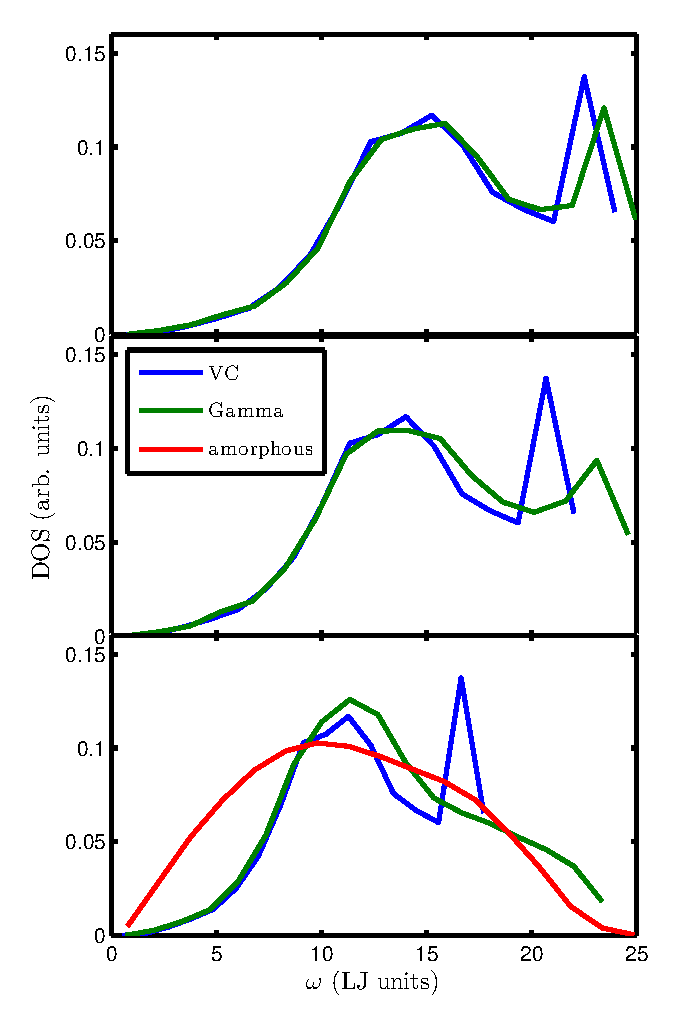
\includegraphics[scale=0.7]
{/home/jason/disorder/lj/alloy/lj_alloy_dos_c05-5_3.eps}
\vspace*{-5mm}
\end{center}
\caption{\label{FIG:phonon_diff} virtual crystal results}
\end{figure}
%--------------------------------------------------------------------------

%--------------------------------------------------------------------------
\subsection{\label{S:}Structure Factor of Gamma Point Modes}
%--------------------------------------------------------------------------

\begin{equation}\label{EQ:M:EL}
E^L\kv = 
\left|
\sum_{l,b} 
\hat{\mathbf{\kappa}} \cdot e\kvba 
\EXP{i\pmb{\kappa}\cdot\mathbf{r}_0\ab{l}{b}} 
\right|^2
\end{equation}

\begin{equation}\label{EQ:M:EL}
E^T\kv = 
\left|
\sum_{l,b} 
\hat{\mathbf{\kappa}} \times e\kvba 
\EXP{i\pmb{\kappa}\cdot\mathbf{r}_0\ab{l}{b}} 
\right|^2
\end{equation}

\begin{equation}\label{EQ:M:SL}
S^{L,T}\kw = 
\sum_{\nu} E^{L,T}\kv
\delta (\omega-\omega\kv)
\end{equation}

Demonstrates the importance of dispersion, even along different lattice 
directions ([100 vs [111]) and polarizations ($S^L,T$).

With increasing concentration, the structure factor spreads in width,  
particularly at high frequencies.  The VC mass becomes larger and the 
peaks in the structure factor shift to lower frequencies. 

An effective dispersion can be extracted by locating the peaks in the 
structure factors, where the effects of polarization, virtual mass, and 
anisotropic dispersion can be detected. The frequencies extracted from 
the structure factors agree with the VC predictions to within less than 
3$\%$. From the dispersion, the mode group velocities can be predicted 
(see Section ), which is necessary to predict thermal conductivity 
(see Section ).

Duda shows the reduction in group velocity of disordered systems.
\cite{duda_reducing_2011}

%--------------------------------------------------------------------------
\begin{figure}
\begin{center}
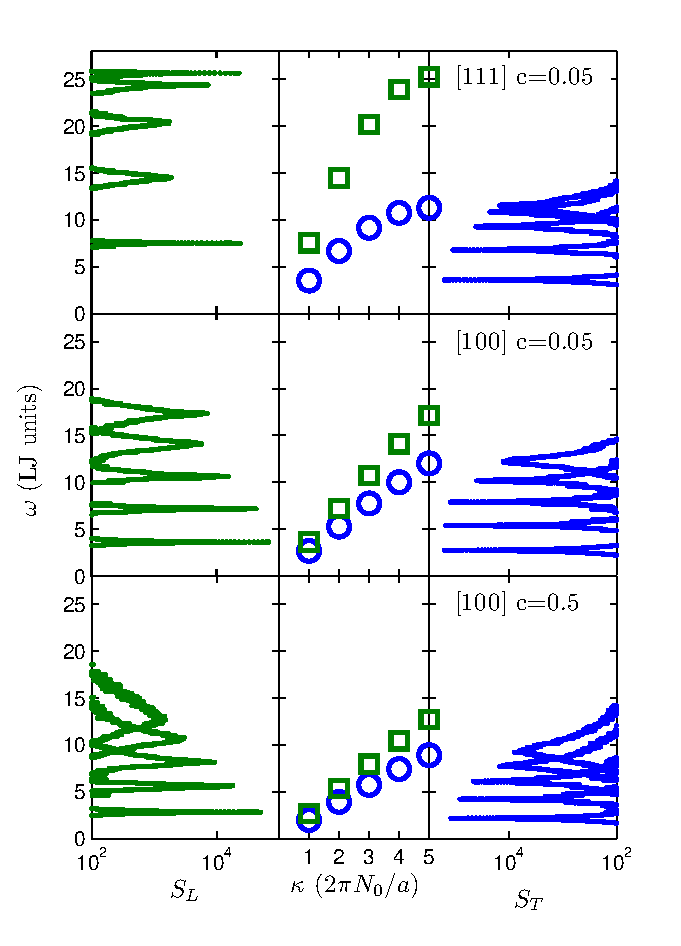
\includegraphics[scale=0.7]
{/home/jason/disorder/lj/alloy/lj_alloy_dsf_100_111.eps}
\vspace*{-5mm}
\end{center}
\caption{\label{FIG:phonon_diff} virtual crystal results}
\end{figure}
%--------------------------------------------------------------------------

%--------------------------------------------------------------------------
\subsection{\label{S:}Phonon Lifetimes}
%--------------------------------------------------------------------------

\begin{equation}\label{EQ:M:tau_matthiessen}
\frac{1}{\tau\kv} = \frac{1}{\tau_{p-p}\kv} + \frac{1}{\tau_{d}\kv},
\end{equation}
where $\tau_{p-p}\kv$ accounts for phonon-phonon scattering,
accounts for boundary scattering, $\tau_{d}\kv$ accounts for defect 
scattering.

Phonon-phonon scattering ($\tau_{p-p}\kv$) is typically treated 
using anharmonic perturbation theory including only 3-phonon 
processes.\cite{turney_predicting_2009,garg_role_2011,tian_phonon_2012} 
It has been estimated that the effects of higher order phonon 
processes are small \cite{ecsedy_thermal_1977}.
At low frequencies,
$\tau_{p-p}\kv$ follows a scaling due to both normal ($B_1\omega^2$) 
and umklapp ($B_2\omega^2$) 3-phonon scattering processes, where 
the density of states is Debye-like. The 
constants $B_1$ and $B_2$ are typically fit to experimental data.

Using harmonic perturbation theory, Tamura gives a general expression 
for mass point defect scattering \cite{tamura_isotope_1983}
\begin{equation}\label{EQ:M:tau_d}
\begin{split}
\frac{1}{\tau_{d}\kv} = \frac{\pi}{2N}\omega\kv^2 
\sum_{\mathbf{\kappa'}\nu'} \delta( \omega\kv - 
\omega\kvp ) \\
\sum_{b} g(b) 
|e^*\kvbap \cdot e\kvba |^2 ,
\end{split}
\end{equation}
where 
$g(b) = \sum_i c_i(b)(1-m_i(b)/\bar m(b))^2,$
N is the number of unit cells. and $c_i$ is the fraction, $m_i$ is the mass, 
and $\bar m_i$ is the average mass of the i-th species.

For the simple single species systems considered in this work, 
$\frac{1}{\tau_{d}\kv} =\frac{\pi}{2} g \omega\kv^2 D(\omega\kv)$, where 
$D(\omega\kv)$ is the density of states. Under the Debye-approximation, 
the phonon scattering due to mass point-defects 
is given by $A\omega^{-4}$, where $A$ is a constant related to the unit 
cell volume, branch-averaged group velocity, and disorder coupling strength 
($g$ in Eq. above). The frequency dependence ($\omega^4$) is the same as 
Rayleigh scattering, which is valid at low frequency where the Debye 
approximation is valid.

Bond disorder 
can be accounted for using a similar expression with an average
atomic radius or suitable scattering cross-section.
\cite{klemens_scattering_1955,klemens_thermal_1957} 
The effect of bond and mass disorder has been investigated computationally 
by Skye and 
Schelling for Si/Ge \cite{skye_thermal_2008}, 
where it was shown that mass disorder is 
the dominant scattering mechanism. In this work we consider only 
mass disorder.

While the
expression for harmonic defect scattering (Eq.) is valid for
perturbative disorder, its use leads to good agreement with
several experimental and computational results with large disorder.  
Cahill shows that conductivty reduction in dilute 
Ge-doped Si epitaxial layers 
is captured mostly by the mass disorder.\cite{cahill_thermal_2005} 
In this case, the mass disorder is large ($m_{Ge}/m_{Si} = 2.6$) 
but the overall disorder strength is dictated by the concentration. 
For example, as little as $6.2\times10^{19} cm^{-3}$ Ge
($g = 3.1\times10^{-3}$) is enough to reduce the thermal conductivity of 
Si by almost a factor of 2.\cite{cahill_thermal_2004}
Even in the
case of the $Ni_{0.55}Pd_{0.45}$ alloy, the atomic species
are chemically similar but both the mass disorder 
($m_{Pd}/m_{Ni} \approx 2$) and concentration are large ($g=0.078$) 
and good agreement is seen with the Eq..
\cite{kamitakahara_vibrations_1974}

Computational results 
\cite{turney_predicting_2009,garg_role_2011,tian_phonon_2012}


%--------------------------------------------------------------------------
\section{\label{S:}Phonon Lifetime Predictions}
%--------------------------------------------------------------------------

%--------------------------------------------------------------------------
\subsection{\label{S:Lifetimes}Normal Mode Decomposition (NMD)}
%--------------------------------------------------------------------------

We use the normal mode decomposition (NMD) method 

 The phonon lifetime is predicted using the following

\begin{equation}\label{EQ:M:tau_d}
\tau\kv = \int_{0}^{\infty} \frac{<E\kvt E\kvzero>}{ <E\kvzero E\kvzero> }dt
\end{equation}

The phonon normal mode coordinates, $q\kvt and qdot\kvt$, are required 
to calculate the phonon normal mode energy $E\kv(t)$. The phonon mode 
eigenvectors, $e\kvba$, are required to map the atomic coordinates onto 
the phonon normal modes. Under the VC approximation, the phonon eigenvectors 
are those of pure plane-waves. In a disordered supercell, the vibrational 
modes are not purely plane-wave (phonon) (see Section) and exist at the 
Gamma point ([000]). Both cases are compared in the next section.

%--------------------------------------------------------------------------
\subsection{\label{S:Lifetimes}VC-NMD and Gamma Point Phonon Lifetimes}
%--------------------------------------------------------------------------

%--------------------------------------------------------------------------
\begin{figure}
\begin{center}
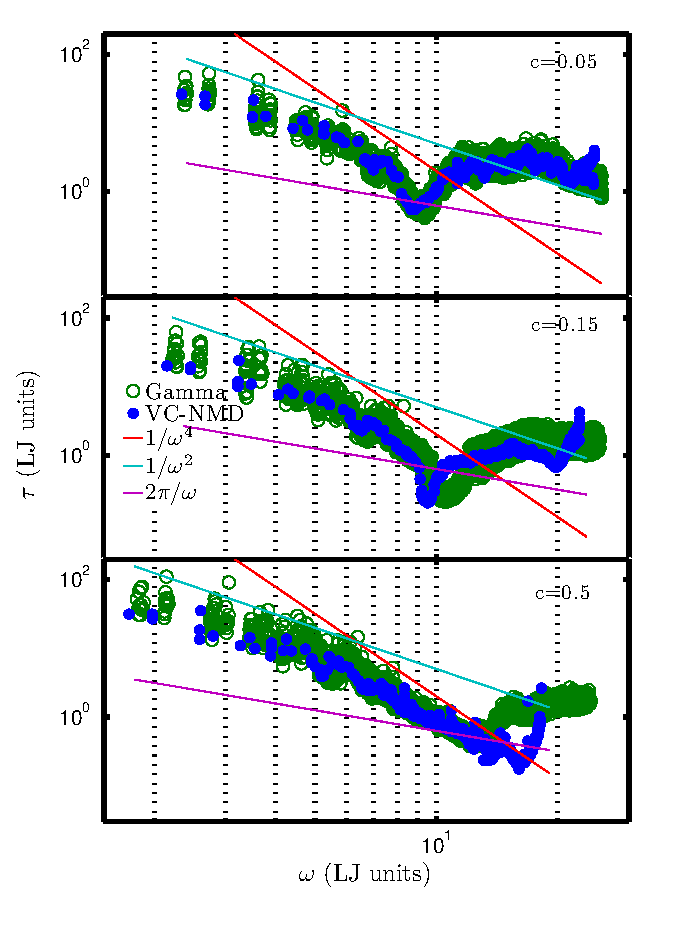
\includegraphics[scale=0.7]
{/home/jason/disorder/lj/alloy/lj_alloy_ald_nmd_vc_gamma_life.eps}
\vspace*{-5mm}
\end{center}
\caption{\label{FIG:phonon_diff} virtual crystal results}
\end{figure}
%--------------------------------------------------------------------------

Gamma refers to mapping using the eigenvectors of the exact harmonic 
eigenmdoes of the disordered supercell. 

eigenvector mappings \cite{koker_thermal_2009}
\cite{qiu_molecular_2011} use NMD to predict the phonon properties of 
PbTe using a classical model.
\cite{shiomi_thermal_2011} half-huesler usese $\Phi'$ and ALD, find good 
agreement. \cite{thomas_predicting_2010} finds increased scattering in 
water-filled CNTs. \cite{ong_reduction_2011} finds increased scattering 
of phonons in CNTs on a substrate. 

In these studies, the atomic coordinates are being mapped onto modes which 
are not eigenmodes of the system's Hamiltonian. Still, the spectral widths 
(inverse lifetimes) of these mappings contain information about the 
scattering time scales associated with these modes.   

%--------------------------------------------------------------------------
\subsection{\label{S:}VC-NMD and VC-ALD Lifetime Comparison}
%--------------------------------------------------------------------------
Essentially, the normal mode mappings are performed using eigenvectors 
which are plane waves.\cite{}

%--------------------------------------------------------------------------
\begin{figure}
\begin{center}
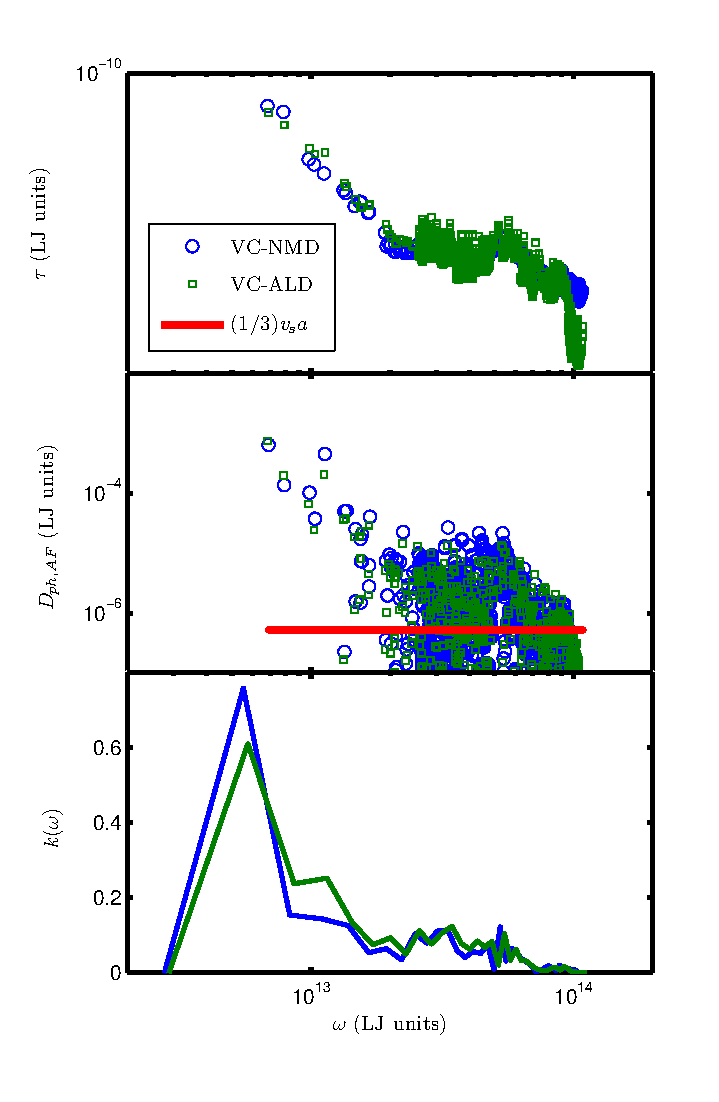
\includegraphics[scale=0.7]
{/home/jason/disorder/lj/alloy/af_nmd_ald_tau_diff_kw_c05.eps}
\vspace*{-5mm}
\end{center}
\caption{\label{FIG:phonon_diff} gamma point results}
\end{figure}
%--------------------------------------------------------------------------

%--------------------------------------------------------------------------
\begin{figure}
\begin{center}
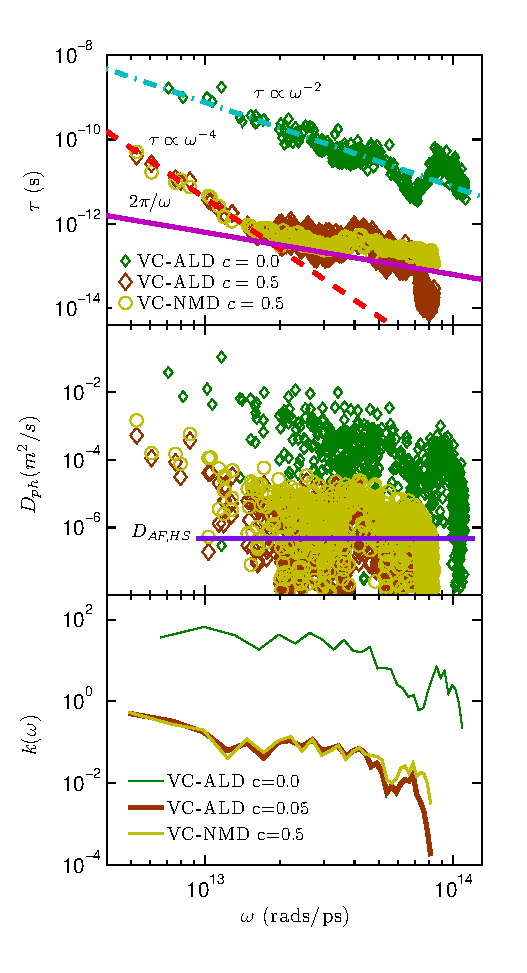
\includegraphics[scale=0.7]
{/home/jason/disorder/lj/alloy/af_nmd_ald_tau_diff_kw_c5.eps}
\vspace*{-5mm}
\end{center}
\caption{\label{FIG:phonon_diff} gamma point results}
\end{figure}
%--------------------------------------------------------------------------

%--------------------------------------------------------------------------
\subsection{\label{S:}Mode Diffusivity}
%--------------------------------------------------------------------------

The high scatter limit is given as:

\begin{equation}\label{EQ:M:k_HS}
k_{CP,HS} = (\frac{\pi}{6})^{1/3} (\frac{3}{2}) \frac{k_{B}}{V_b}b v_s a
\end{equation}

where $V_b$ is the volume of the unit cell, $v_s$ is the 
branch-averaged sound speed, and $a$ is the lattice constant 
(or appropriate length scale).\cite{cahill_lattice_1988} 
The characteristic diffusivity of each mode in the 
high-scatter limit is
\begin{equation}\label{EQ:M:k_HS}
D_{CP,HS} = 0.403 v_s a.
\end{equation}
where the vibrational mode MFP is taken to be $a$.

From the disordered harmonic theory of Allen-Feldman (referred to as AF), 
the thermal conductivity in the high-scatter limit can be written as
%\begin{equation}\label{EQ:M:k_HS}
%k_{AF,limit} = sum_i^{modes}  (kb/V) \frac{1}{3} v_s a  =  k_{B} n_v v_s a
%\end{equation}
\begin{equation}\label{EQ:M:k_HS}
k_{AF,HS} = \sum_i^{modes}  \frac{k_{B}}{V} D_{AF,HS}
\end{equation}

where the characteristic diffusivity of each mode in the 
high-scatter limit is

\begin{equation}\label{EQ:M:k_HS}
D_{AF,HS} = \frac{1}{3} v_s a.
\end{equation}

Comparing with Eq., the AF HS limit predicts a mode diffusivity and 
thermal conductivity which is $\%20$ smaller.\cite{cahill_lattice_1988} 

%--------------------------------------------------------------------------
\begin{figure}
\begin{center}
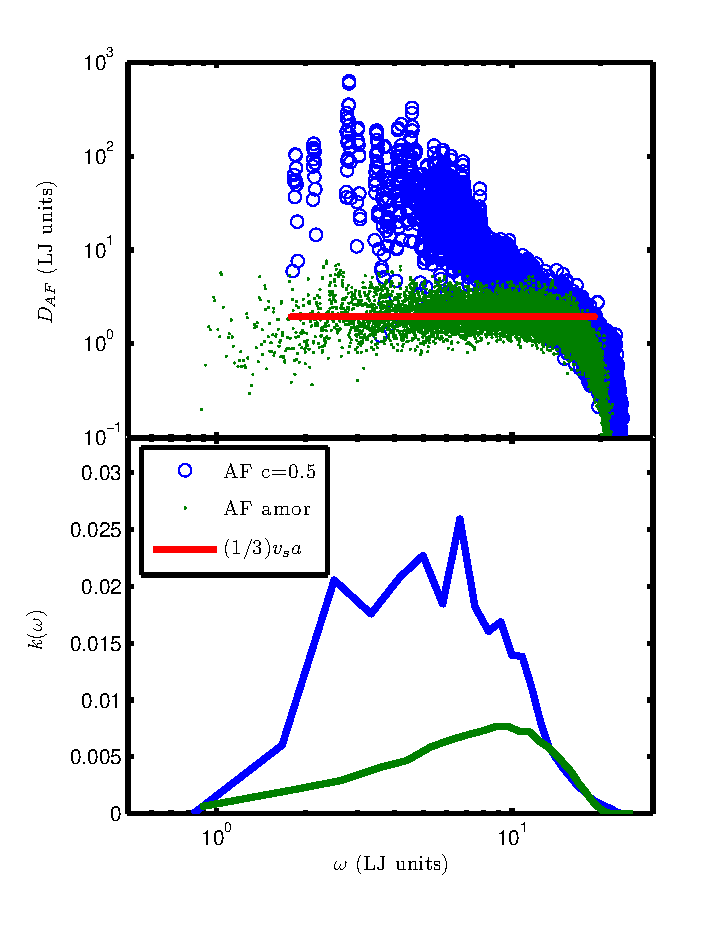
\includegraphics[scale=0.7]
{/home/jason/disorder/lj/alloy/af_c5_amor_DAF_kw.eps}
\vspace*{-5mm}
\end{center}
\caption{\label{FIG:phonon_diff} gamma point results}
\end{figure}
%--------------------------------------------------------------------------

%--------------------------------------------------------------------------
\section{\label{S:Lifetimes}Thermal Conductivity Predictions}
%--------------------------------------------------------------------------

An addition of as little as 10\% Ge is sufficient to reduce the thermal 
conductivity to the minimum value achievable through alloying. 
Theoretically, mass disorder is found to increase the 
anharmonic scattering of phonons 
through a modification of their vibration eigenmodes. 
Notably, the thermal conductivity is found
to drop sharply after only a small amount of alloying. This
is due to the strong harmonic scattering of phonons even
in the dilute alloy limit.

Duda shows that taking a perfect alloy and disordering via an order 
parameter allows control of thermal conductivity.
\cite{duda_controlling_2012}

The thermal conductivity of amorphous solids at low temperatures contain 
quantum statistical effects.\cite{freeman_thermal_1986} Molecular dynamics 
simulations are not able to capture quantum statistical effects.

%--------------------------------------------------------------------------
\begin{figure}
\begin{center}
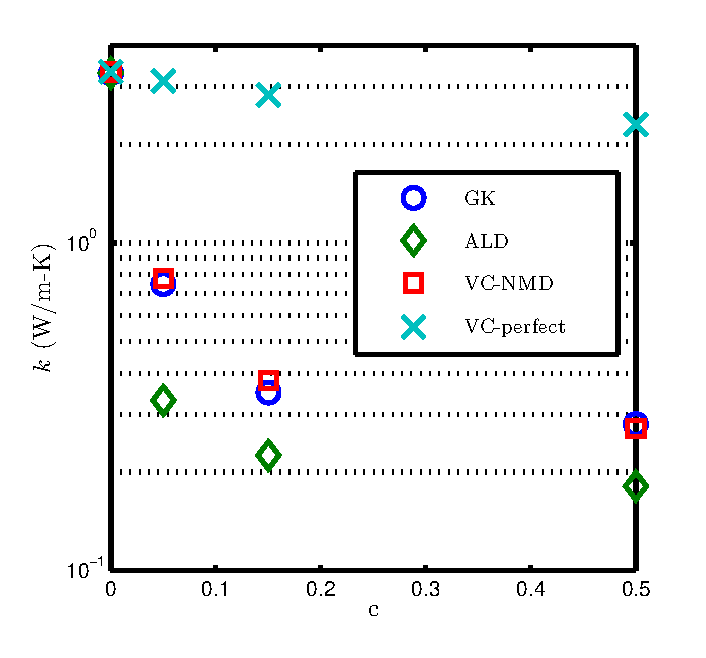
\includegraphics[scale=0.7]
{/home/jason/disorder/lj/alloy/lj_alloy_cond_gk_vc_ald_compare.eps}
\vspace*{-5mm}
\end{center}
\caption{\label{FIG:gk_alloy} The vibrational conductivity of LJ alloys 
predicted using MD simulations and the Green-Kubo method. The predicted 
thermal conductivities are for a LJ alloy of the form $m^a_{1-c}m^b_{c}$, 
where $m^a =$ 1, $m^b=$ 3, and $m_r = m^a/m^b=$ 3 (in LJ units). As the 
alloy concentration is increased perturbatively, the vibrational 
conductivity drops quickly and saturates to a minimum at $c=0.5$. For 
$c=0.5$ the system is heavily disordered and the vibrational conductivity 
approaches that of an amorphous system.}
\end{figure}
%--------------------------------------------------------------------------

%--------------------------------------------------------------------------
\begin{figure}
\begin{center}
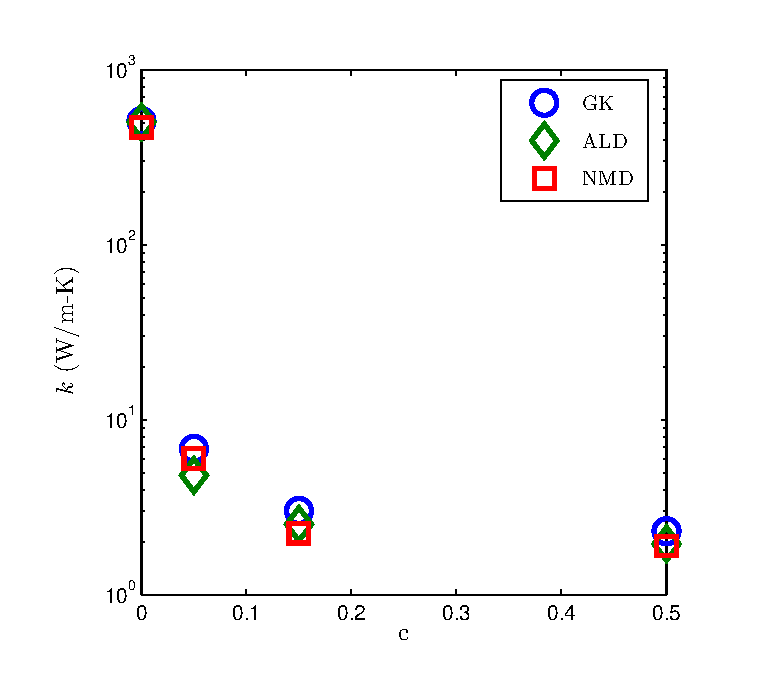
\includegraphics[scale=0.7]
{/home/jason/disorder/si/alloy/si_alloy_cond_gk_vc_ald_compare.eps}
\vspace*{-5mm}
\end{center}
\caption{\label{FIG:gk_alloy} The vibrational conductivity of LJ alloys 
predicted using MD simulations and the Green-Kubo method. The predicted 
thermal conductivities are for a LJ alloy of the form $m^a_{1-c}m^b_{c}$, 
where $m^a =$ 1, $m^b=$ 3, and $m_r = m^a/m^b=$ 3 (in LJ units). As the 
alloy concentration is increased perturbatively, the vibrational 
conductivity drops quickly and saturates to a minimum at $c=0.5$. For 
$c=0.5$ the system is heavily disordered and the vibrational conductivity 
approaches that of an amorphous system.}
\end{figure}
%--------------------------------------------------------------------------

VC-NMD and ALD-taud underpredict vs GK by about 20-30, 
while for LJ the underprediction is 2-300





%--------------------------------------------------------------------------
\begin{figure}
\begin{center}
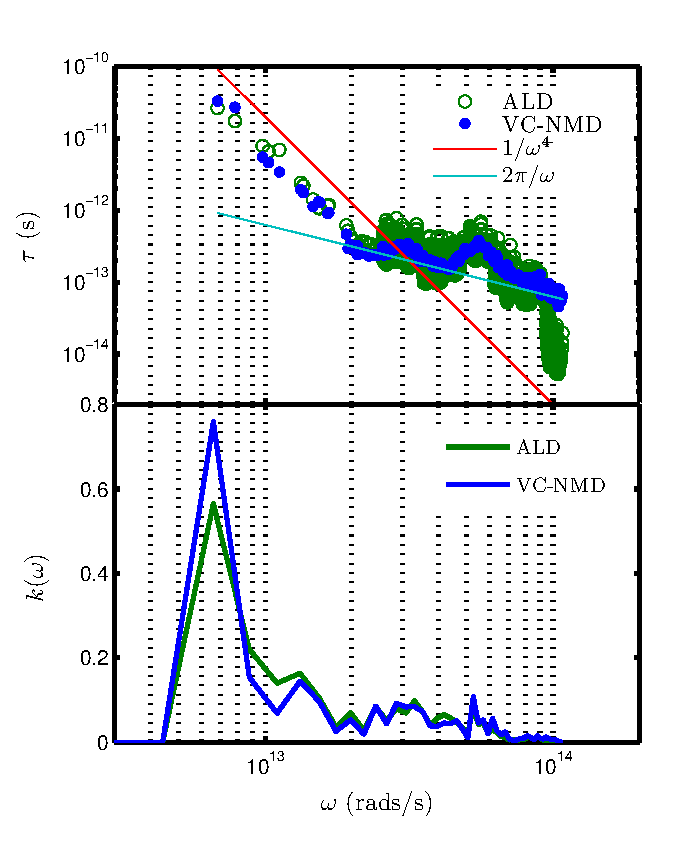
\includegraphics[scale=0.7]
{/home/jason/disorder/lj/alloy/alloy_lj_si_life_kw.eps}
\vspace*{-5mm}
\end{center}
\caption{\label{FIG:phonon_diff} gamma point results}
\end{figure}
%--------------------------------------------------------------------------

%--------------------------------------------------------------------------
\begin{figure}
\begin{center}
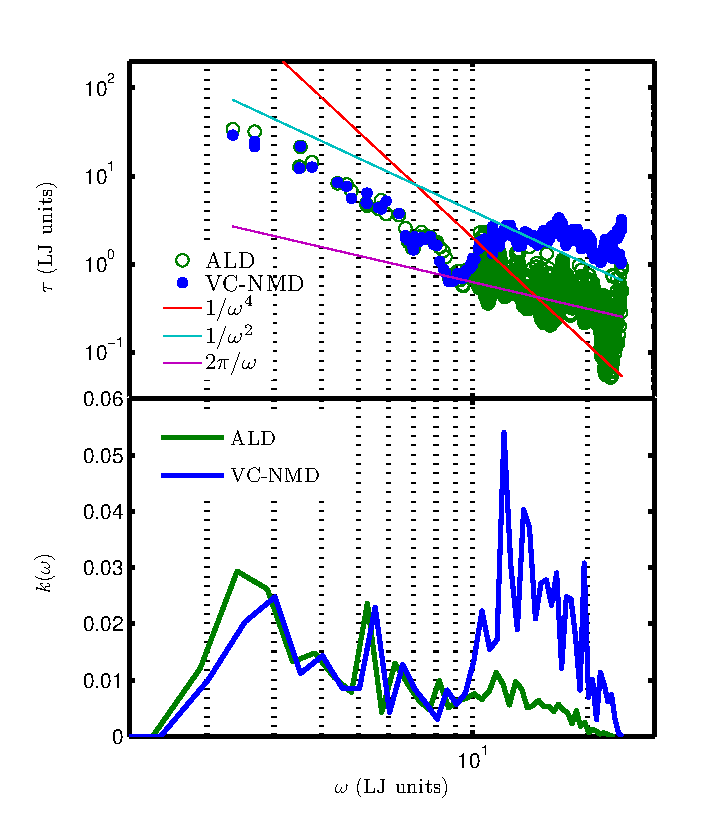
\includegraphics[scale=0.7]
{/home/jason/disorder/lj/alloy/alloy_lj_life_kw.eps}
\vspace*{-5mm}
\end{center}
\caption{\label{FIG:phonon_diff} gamma point results}
\end{figure}
%--------------------------------------------------------------------------


%--------------------------------------------------------------------------
\section{\label{S:}Discussion}
%--------------------------------------------------------------------------

the problem is with taud.  VC-NMD agrees well with GK for both LJ and SW, 
while ALD-taud underpredcits for LJ.  VC-NMD and ALD-taud use the same 
group velocity and classical specific heat.

For diffusons, one can still assign a mfp by the following:

%--------------------------------------------------------------------------
\subsection{\label{S:}Boundary Scattering}
%--------------------------------------------------------------------------
Boundary scattering is responsible for decreasing the long lifetimes 
(mean free paths) of low frequency phonons which carry a significant 
amount of heat, making it particularly effective at decreasing the 
thermal conductivity of systems with length scale of 100s of nm and 
less.\cite{mcgaughey_nanostructure_2012}

First-principles calculations on some thermoelectric
materials show that phonons have a wide MFP distribution,
and hence relatively large nanostructures can reduce their
lattice thermal conductivity.5,18,19 On the other hand, recent
first-principles calculations have shown that the distribution is
much narrower for PbTe,20 and thus, further characterizations
of the distributions and the associated detailed heat conduction
of lead chalcogenides are important for better material design.
%--------------------------------------------------------------------------
\section{\label{S:}Summary}
%--------------------------------------------------------------------------


%--------------------------------------------------------------------------
\appendix
%--------------------------------------------------------------------------


\section{\label{A-Allowed-Wavevectors-Ordered}Allowed Wavevectors in 
Ordered and Disordered Systems}
%--------------------------------------------------------------------------
The phonon spectral energy is defined for the allowed wavevectors of a 
crystal, which can be specified from the crystal structure's Bravais 
lattice and its basis, i.e. unit cell. A $D$-dimensional Bravais lattice 
is a collection of points with
positions
\begin{equation}\label{crys_pos}
\begin{split}
\mathbf{u}_0\ab{l}{0} =& \sum^D_{\alpha} N_{\alpha}\mathbf{a}_{\alpha}
\end{split}
\end{equation}
where $N_{\alpha}$ and the summations if over the lattice vectors, 
$\mathbf{a}_{\alpha}$.\cite{ashcroft1976} The basis (or unit cell) is the 
building block of the crystal and they are arranged on the points defined 
by the Bravais lattice. The equillibrium position of any atom in the crystal 
can be described by
\begin{equation}\label{crys_pos2}
\begin{split}
\mathbf{u}_0\ab{l}{b} = \mathbf{u}_0\ab{l}{0} + \mathbf{u}_0\ab{0}{b}
\end{split}
\end{equation}
where $\mathbf{u}_0\ab{l}{0}$ is the equilibrium position of the 
$l^{\textrm{th}}$ unit cell and $\mathbf{u}_0\ab{0}{b}$ is the equilibrium 
position of the and $b^{\textrm{th}}$ atom in the unit cell relative to 
$\mathbf{u}_0\ab{l}{0}$.
For the LJ systems studied here, the cubic conventional cells are used with 
four atoms per unit cell.\cite{ashcroft1976} For our MD simulations, cubic 
simulation domains with periodic boundary conditions are used with 
$N_1 = N_2 = N_3 = N_0$.\cite{turney2009a,mcgaughey2004a} The allowed 
wavevectors for such crystal structures are
\begin{equation}\label{crys_pos3}
\begin{split}
\pmb{\kappa} = \sum_{\alpha} \mathbf{b}_{\alpha} 
\frac{n_{\alpha}}{N_{\alpha}},
\end{split}
\end{equation}
where $\mathbf{b}_{\alpha}$ are the reciprocal lattice 
vectors\cite{ashcroft1976} and $-N_{\alpha}/2 < n_{\alpha} 
\leq N_{\alpha}/2$, where $n_{\alpha}$ are integers and $N_{\alpha}$ 
are even integers.\cite{turney2009a} The wavevectors are taken to be 
in the first Brioullin zone.\cite{ashcroft1976}

Strictly speaking, the only allowed wavector in a disordered system is the 
gamma point ($\kappa = [0 0 0]$). As such, the lattice dynamics calculations 
are performed at the gamma point:

%--------------------------------------------------------------------------
\subsection{\label{S:Lifetimes:}Normal Mode Decomposition}
%--------------------------------------------------------------------------
If $\gamma \kv > \omega \kv$, then the vibrational mode is overdamped.  
Discuss why real-space method is necessary in this case.
%--------------------------------------------------------------------------
\section{\label{A-Finite-Sim}Finite Simulation-Size Scaling for Thermal 
Conductivity}
%--------------------------------------------------------------------------
For the LJ argon system studied in Section \ref{S-Prelim-Vib-Cond-Ordered}, 
a finite simulation-size scaling procedure\cite{turney2009a,He2011a} is 
used to compare the thermal conductivity predictions from $\Phi$ and $\Phi'$ 
to those from the Green-Kubo method. The scaling procedure is demonstrated in 
Fig$.$ \ref{FIG:LJ_COND}. The thermal conductivity is predicted from $\Phi$ 
or $\Phi'$ and MD simulations with $N_0 = 4,6,8,$ and $10$. The bulk 
conductivity, $k_{\infty}$, is then estimated by fitting the data to
\begin{equation}\label{k_size}
\begin{split}
1/k = 1/k_{\infty} + A/N_0,
\end{split}
\end{equation}
where $A$ is a constant. This procedure is necessary because the first 
Brillouin zone is only sampled at a finite number of points for a finite 
simulation size, with no contribution from the volume at its center. To 
predict a bulk thermal conductivity, it is important to sample points near 
the Brillouin zone center, where the modes can have large lifetimes and 
group velocities.\cite{turney2009a,sellan2010b} 


\clearpage
\bibliographystyle{apsrev}
\bibliography{/home/jason/ntpl-ref/ntpl-jason/ntpl-jason-111512}
\end{document}
